\documentclass[psamsfonts]{amsart}

%-------Packages---------
\usepackage{amssymb,amsfonts}
\usepackage[all,arc]{xy}
\usepackage{enumerate}
\usepackage{mathrsfs}
\usepackage{xcolor}
\usepackage{graphicx}
%--------Theorem Environments--------
%theoremstyle{plain} --- default
\newtheorem{thm}{Theorem}[section]
\newtheorem{cor}[thm]{Corollary}
\newtheorem{prop}[thm]{Proposition}
\newtheorem{lem}[thm]{Lemma}
\newtheorem{conj}[thm]{Conjecture}
\newtheorem{quest}[thm]{Question}

\theoremstyle{definition}
\newtheorem{defn}[thm]{Definition}
\newtheorem{defns}[thm]{Definitions}
\newtheorem{con}[thm]{Construction}
\newtheorem{exmp}[thm]{Example}
\newtheorem{exmps}[thm]{Examples}
\newtheorem{notn}[thm]{Notation}
\newtheorem{notns}[thm]{Notations}
\newtheorem{addm}[thm]{Addendum}
\newtheorem{exer}[thm]{Exercise}

\theoremstyle{remark}
\newtheorem{rem}[thm]{Remark}
\newtheorem{rems}[thm]{Remarks}
\newtheorem{warn}[thm]{Warning}
\newtheorem{sch}[thm]{Scholium}

\makeatletter
\let\c@equation\c@thm
\makeatother
\numberwithin{equation}{section}

\bibliographystyle{plain}

%--------Meta Data: Fill in your info------
\title{Gamma-Cross Sections} 

\author{Zo\"e Smith}


\date{DEADLINES: Draft AUGUST 19 and Final version AUGUST 31, 2019}

\begin{document}
\begin{center}
	{\bfseries Modifying Number of Terms Calculated \\in DFT can Increase Accuracy}\\
	Zo\"e Smith
\end{center}

 \section{Statement}
 In this project I investigated was how the does increasing the number of terms calculated in an iDFT while keeping the number evaluations in a Discrete Fourier Transform (DFT) impact the accuracy of an approximation of an image. 
 
 There are many applications to this project. Too start, approximations by Fourier transforms are very common in signal processing done in communications. Fourier transformations are also common in JPEGs, which use Fourier Transforms in both dimensions of the image to store it. From an artistic viewpoint, modeling images by Fourier transforms allow us a means to visualize and quantize abstraction. Fourier Transforms of images via parametrizations are also very common in animations, so understanding the mechanisms behind these animations is also incredibly valuable. 
 \section{Project Objective}:
 \begin{itemize}
 	\item Were accurate approximations of images using Fourier Transforms found?
 	\item Was a connection found between number of terms included and similarity to an image?
 \end{itemize}
 
 \section{Relevant Work}
 Joseph Fourier first formalized Fourier transforms in his paper \textit{Analytic Theory of Heat} in 1822. In this paper he used a basis of sinusoidal functions to expand functions and theorized that any function could be expanded as an infinite sequence of such terms. 
 
 In this project, I followed Alex Millers website and GitHub repository [1] to create the parametrization of the image. I also used Jez Swanson's article [2] to understand `An Interactive Introduction to better understand Fourier transforms.
 
\section{Computational Methods}
The methodology for this project was broken down into three stages, the parametrization, taking the Fourier transforms, and comparing the similarity of those Fourier approximations to the parametrization of the image. 

\section{Parametrization}
First, a black and white line drawing was chosen. For this experiment I chose a line drawing of a girl jumping to study as shown in figure 1.

\begin{figure}[h!]
	\centering
	
\includegraphics[scale=.75]{girl.jpg}
	\caption{The original picture of a girl jumping. This was only used to generate a parametrization, and not used at any other point.}
\end{figure}


 All images were handled in this experiment in python as NumPy arrays. A path through the black pixels(indicated by `0' in NumPY arrays). Some manipulation was necessary to ensure that the imported image was strictly black and white and not gray-scale or RBG. The path was set to start and end at the same spot- a feature that would be useful for the Fourier transforms. From this path, SciPy's Univariate Splines function was used to create a parametrization. Univariate Splines approximate the curved path by a lines at increments. The period of our parametrization was fixed by the number of black pixels, `T', in our array. The time step was chosen by setting a number of evaluations- `m.' The Univariate Splines function was used in both the $x$ and $y$ dimensions to get parametrizations $x(t)$ and $y(t)$. 
This parametrization can be plotted to get our `base image' that we will compare our approximations to.  The parametrization shown at step size 250 is shown in figure 2. 

\begin{figure}[h!]
	\centering
	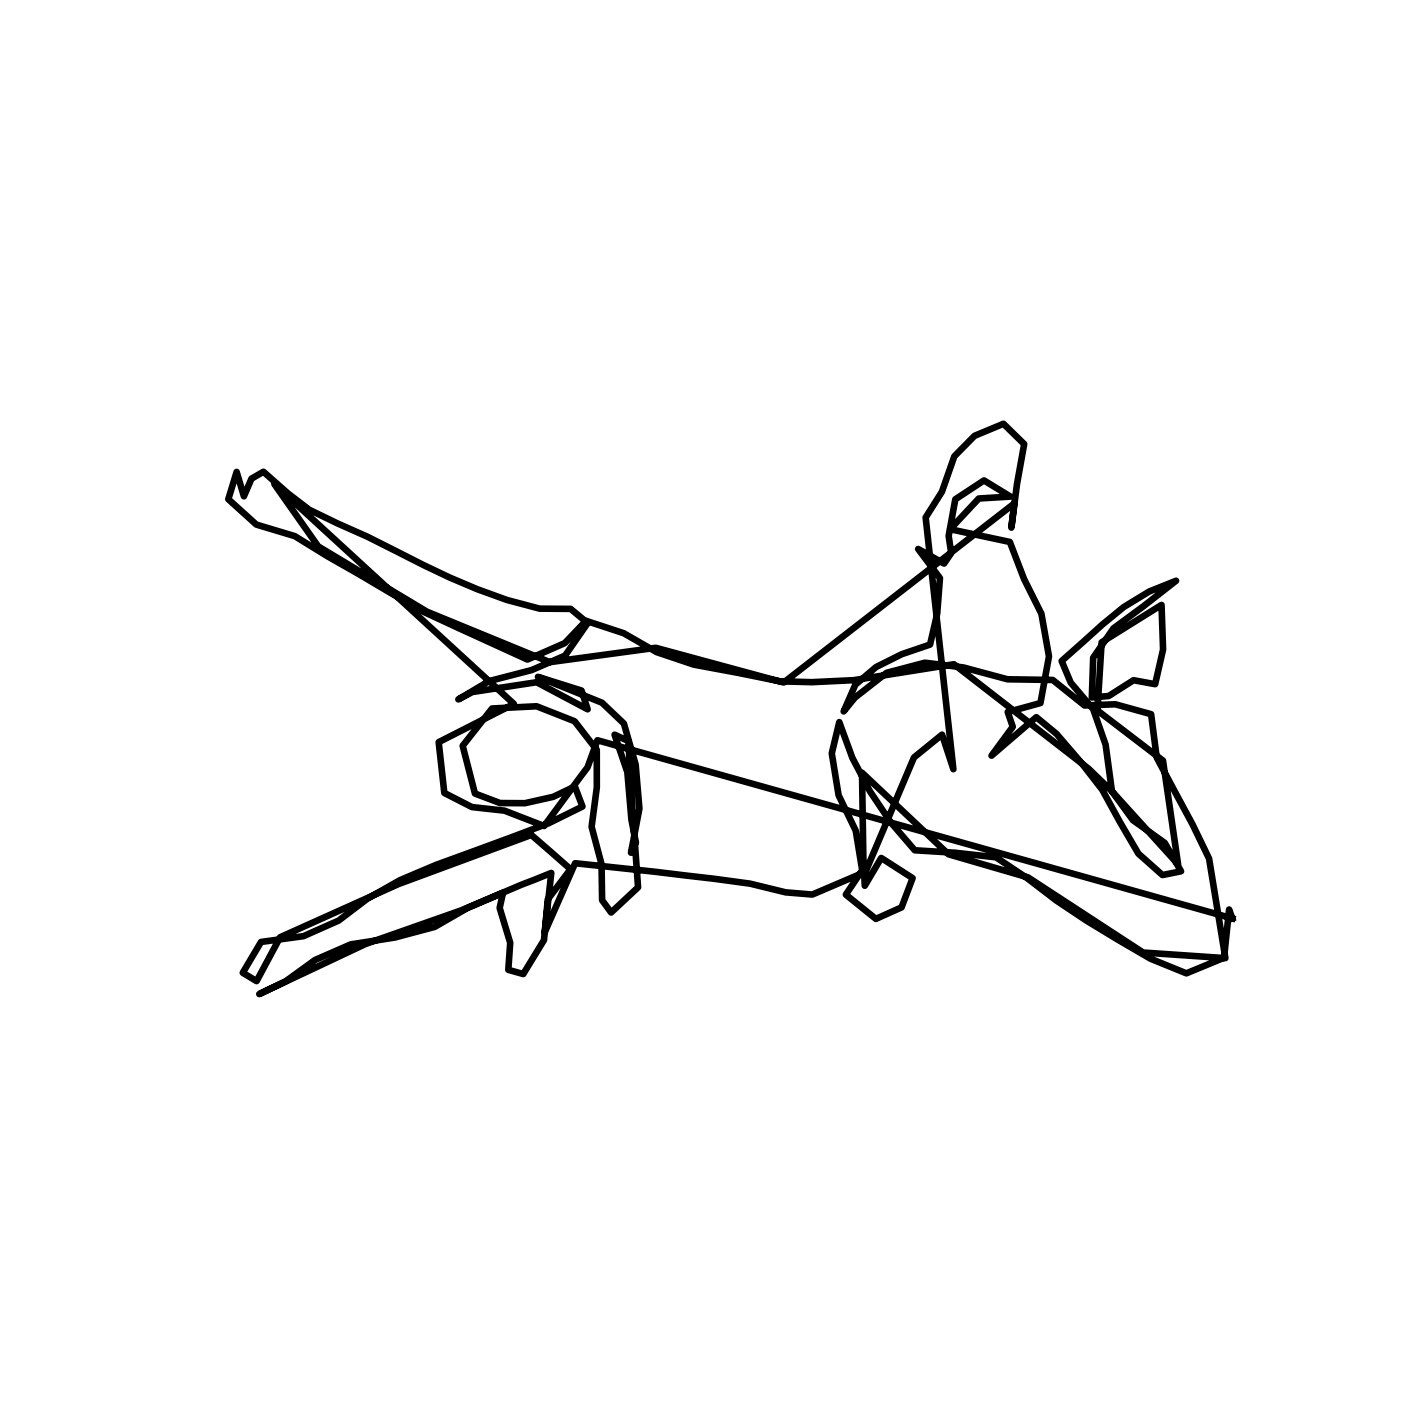
\includegraphics[scale=.2]{girl_250_param.png}
	\caption{The parametrization generated from SciPy Univariate Splines. Used for all comparisons to the Fourier approximations.}
\end{figure}

\subsection{Fourier Transforms}
A discrete Fourier transform was taken for the $x$ and $y$ dimensions they were calculated by the following equations:
\begin{equation}\label{cn}
c_n = \frac{1}{m} \sum_{t=0}^T f(t)e^{{-i2\pi nt}{T}}
\end{equation}
In this equation, $m$ is the number of evaluations taken, $T$ is the period of our function, and the summation runs from $0$ to $T$ in increments of $T/m$.
From these $c_n's$, an inverse DFT was taken to recover an approximation of the 
\begin{equation}\label{ft}
f(t) = \sum_{n=0}^N c_ne^{\frac{i2\pi nt}{T}}
\end{equation}
 where $T$ is the period of our function, $N$ is the number of terms we are evaluating. In this experiment we will vary $N$. Normally, the DFT equation would evaluate $N=m$. By plotting both the approximations of $x(t)$ and $y(t)$ an approximation of our image was found. 
 
\subsection{Image Approximation}:
The similarities between the parameterized image and the approximation of the image by taking the percent similarity.This analysis will not transfer between other images, because the number of white buffer space around the edges will change- `padding' the similarities. This mage is advantageous because it penalizes both over-fitting and under-fitting of the image. Over-fitting is seen when the approximation creates excessive `squiggles' around each line, while under-fitting occurs when the approximation doesn't reach or recreate lines at all. Examples of over-fitting shown in figure 3 and under-fitting is shown in figure 4. 

\begin{figure}[h!]
	\centering
	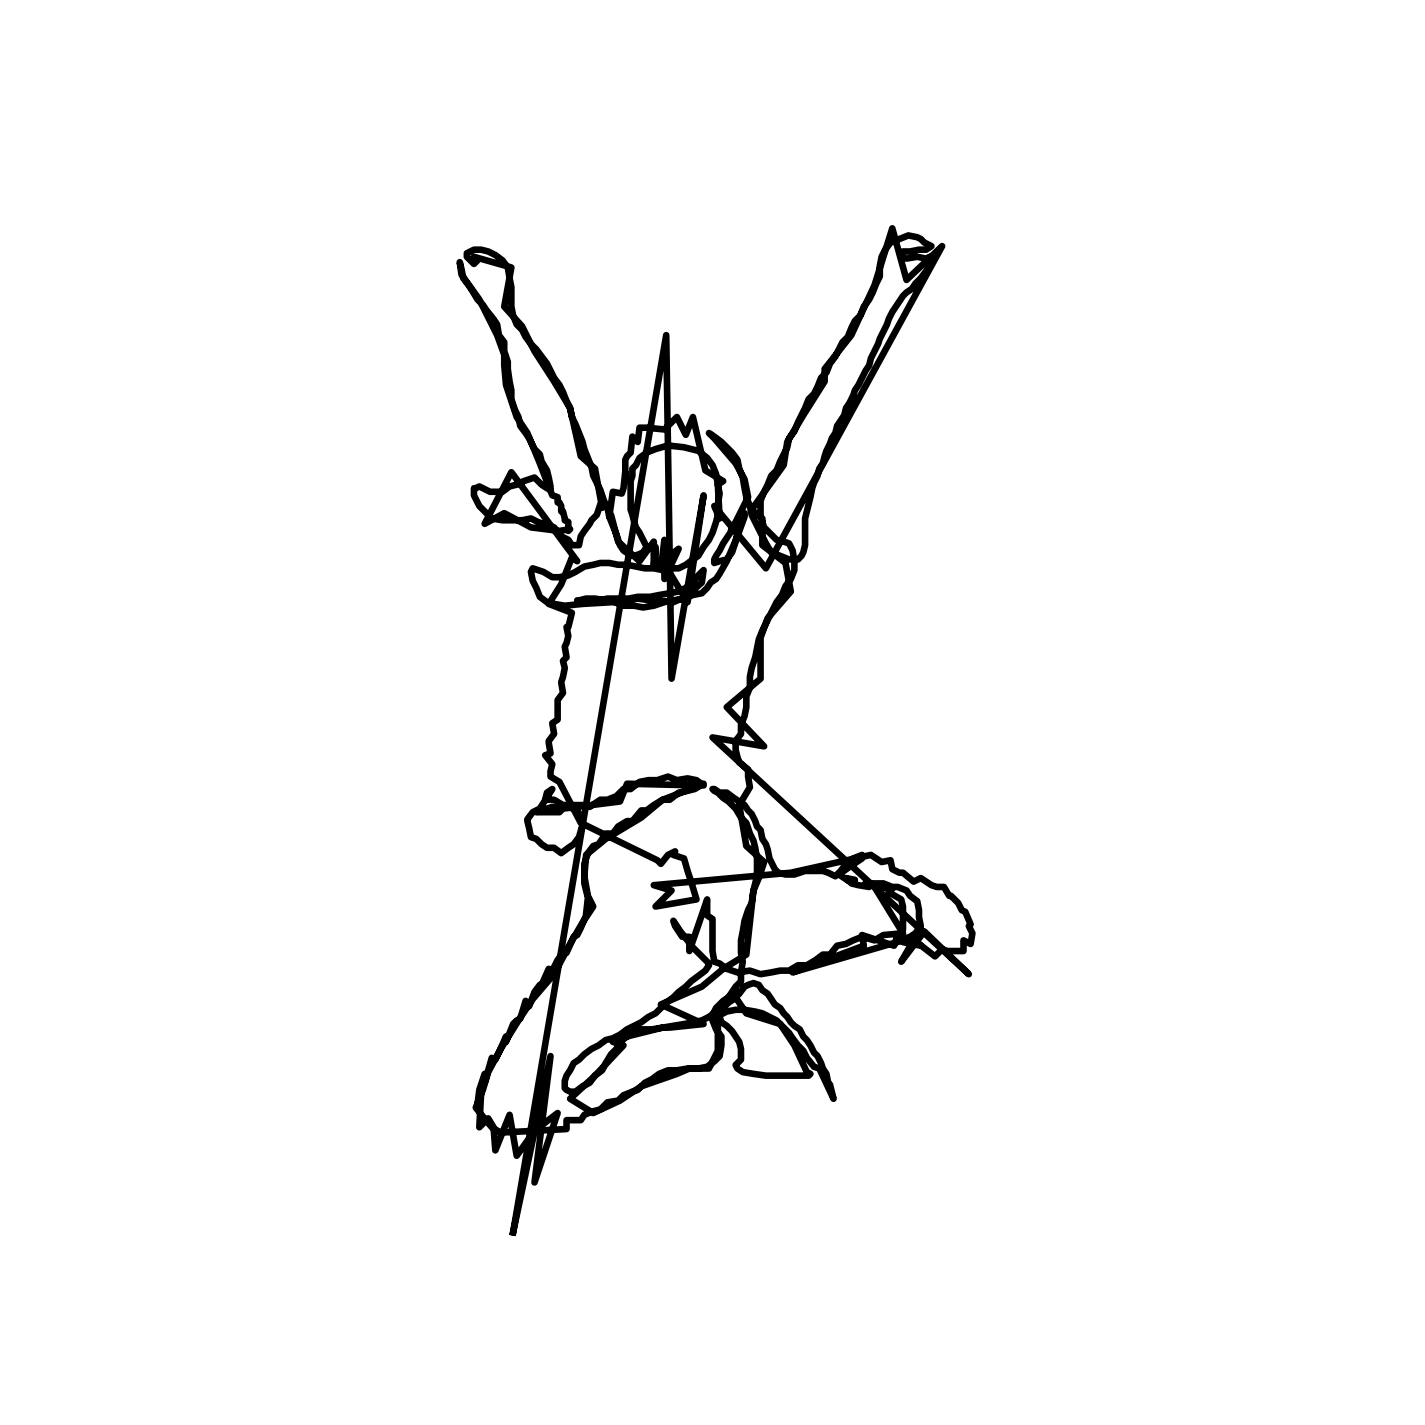
\includegraphics[scale=.2]{girl1220.png}
	\caption{An example of over-fitting. This included 1220 terms of the iDFT, with m=1000.}
\end{figure}

\begin{figure}[h!]
	\centering
	
\includegraphics[scale=.2]{girl12.png}
	\caption{An example of under-fitting. This included 12 terms of the iDFT, with m=1000.}
\end{figure}
Comparing our approximations to the parametrization-a simulation of our originals image- allows us to isolate the strength of the Fourier transform approximation to what it is approximating- the parametrization- and avoid testing the strength of the parametrization to the original image.
By using a parametrization that starts and ends in the same place, we have functions $x(t)$ and $y(t)$ that start and end at the same spot- making them truly periodic. This strengthens application of Fourier transformations that are applied to periodic functions. 

\section{Analysis/Results}
In this experiment we took the spectra of the DFTs at 250, 500, 750, and 1000 evaluations including a range of 2 terms to a couple thousand terms(it changed for each spectrum). We found that these spectra had a periodic nature.In each of these spectra, we were able to approximate the uncertainty with over $99.8\%$ accuracy. With the m=250 spectrum, by calculating the Fourier Approximation including up to 4500 terms, we were able to see four full periods of length $2m$ in spectrum.The spectrum of the for 250 evaluations is included in figure 5.

\begin{figure}[h!]
	\centering
	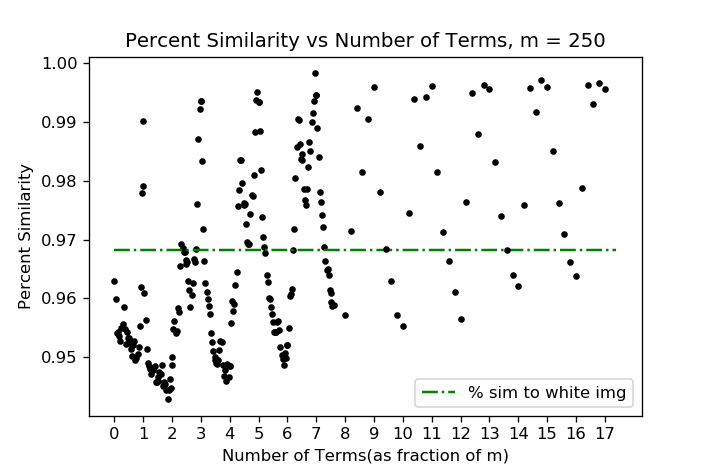
\includegraphics[scale=.5]{girl_250_finalplot.png}
	\caption{For m=250, the spectrum of percent accuracy of image approximation against the number of terms included(N).
	Everything below green line indicates image was less similar than white picture was}
\end{figure}


 I found that the most maximum relative maximums were found within $\pm 2$ terms of every odd multiple of $m$, while there was a patterned oscillation between these values. The relative maxima over the first four periods increases over each period. I estimated the uncertainty in the peaks by considering the growth of the spectra at those points. I optimized a linear fit using the least squares method and found the slope to be $5.5\pm0.9\times 10^{-4}$\%/terms calculated, or when converted to units of $m$,   $0.14 \pm 0.02$ \%/m.This plot is shown in figure 6.
 \begin{figure}[h!]
 	\centering
 	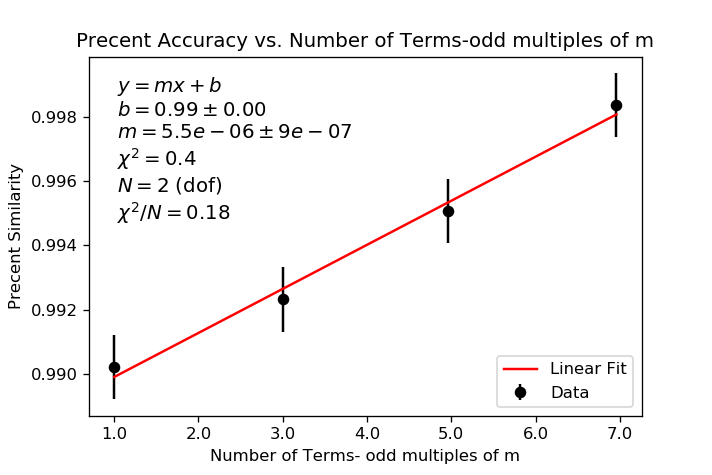
\includegraphics[scale=.4]{girl_250_firstfour.png}
 	\caption{The linear fit of the first four relative maxima for $N$mod $m$ odd.}
 \end{figure}
 
 
  This fit with a reduced chi square of $0.18$ which indicates an overestimation of our uncertainties. This slope indicates a linear increase in the accuracy of our approximation when including terms up to odd  multiples of $m$. This trend cannot go on forever, however. If we were to extrapolate this out to $9m$ terms included, we would have over $100\%$ accuracy! We found when considering the relative maxima at $9m, 11m, 13m$ and $15m$  the slope was negligible with a reduced chi square of $0.9$.  This indicates an extreme overestimation of our uncertainties. This plot can be seen in figure 7. This indicates that the relative maxima even out after 4 periods. 
  
  \begin{figure}[h!]
  	\centering
  	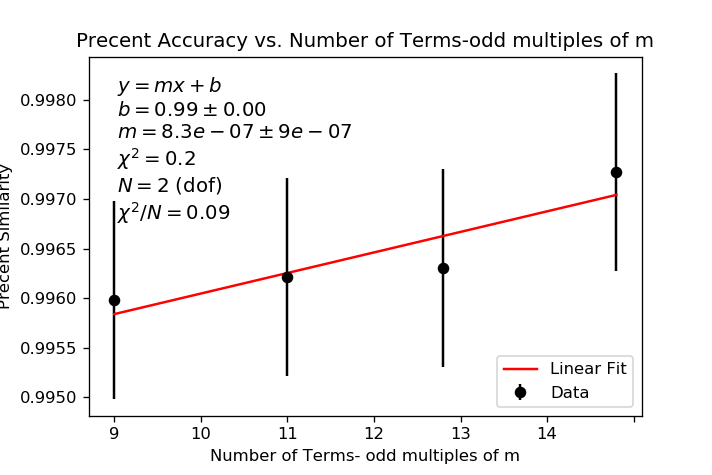
\includegraphics[scale=.4]{girl_250_nextfour.png}
  	\caption{The linear fit of the second four relative maxima for $N$mod $m$ odd.}
  \end{figure}
  

\section{Conclusions}
First, we have found that we can accurately approximate an image with discrete Fourier transforms of the parametrization of the image- with a maximum accuracy of at least $99.8\%$ for each evaluation level($m$) tested. Second, we found that there was a linear increase in the percent accuracy when comparing the accuracy at numbers of terms,$N$, calculated where $$N= am$$ where $a$ is odd and $T/m$ is the time step. This is because the Fourier transform is only plotted in time step increments of $T/m$, this means that the oscillatory function that is added in at each consecutive $N$ will have periods that correspond to the sampling frequency of $m/T$. When this frequency corresponds to be a multiple of $2m/T$, there will be and odd number of crossings per period of the highest frequency sine and cosine added- resulting in an increased accuracy. This implies that by keeping the time step constant and increasing the number of terms calculated in our iDFT, it is possible to increase the accuracy of our image approximation. 

From here, there are many further experiments that could be made. To start, I did not touch the analysis of the non-maximal points in the cycle. There are 3 more relative maxima within each that could be analyzed. I would also be interested in seeing how the spectra change with a more nuanced method of image detection- this could include a system that would consider the distance of black pixels in the `approximation' to the black pixels in the parametrization. Further investigations could be to expand these findings to other images, and compare the optimal number of terms to calculate. Other investigations could also be into the frequencies of the oscillations of the percent similarities, as it is periodic. This would require more Fourier transforms. 



\section{Citations}
[1]$https://github.com/alexmill/website_notebooks$

[2]$http://www.jezzamon.com/fourier/index.html$

\end{document}
